%\addcontentsline{toc}{chapter}{Socio-economical context}
\section{Socio-economical context}

In the past seven years the world has experienced the effects of the recession that appeared in the late 2000s decade. It still affects the economy nowadays and the experts do not know how many more years the situation will stay the same. \\

In Spain the recession has had a big impact that can still be seen in the unemployment numbers and jobs offers. Also, the poverty has increased enormously and the quality of life has decreased together with the salaries.  
\\

There is a general discontent with the politics and the banks. Pessimism is everywhere, as well as the feeling that it is needed a change of direction in both fields. 
\\


This economic context has created and motivated new ways of investigating and living, always aiming at spending as less as possible. It has triggered a change in the perception of the knowledge and whether it should be restricted using patents or not. Most of the scientific community now supports the open source initiative, a fact that has increased the rapidity of the new discoveries and technology improvements. 

\begin{figure}[h]
	\begin{center}
    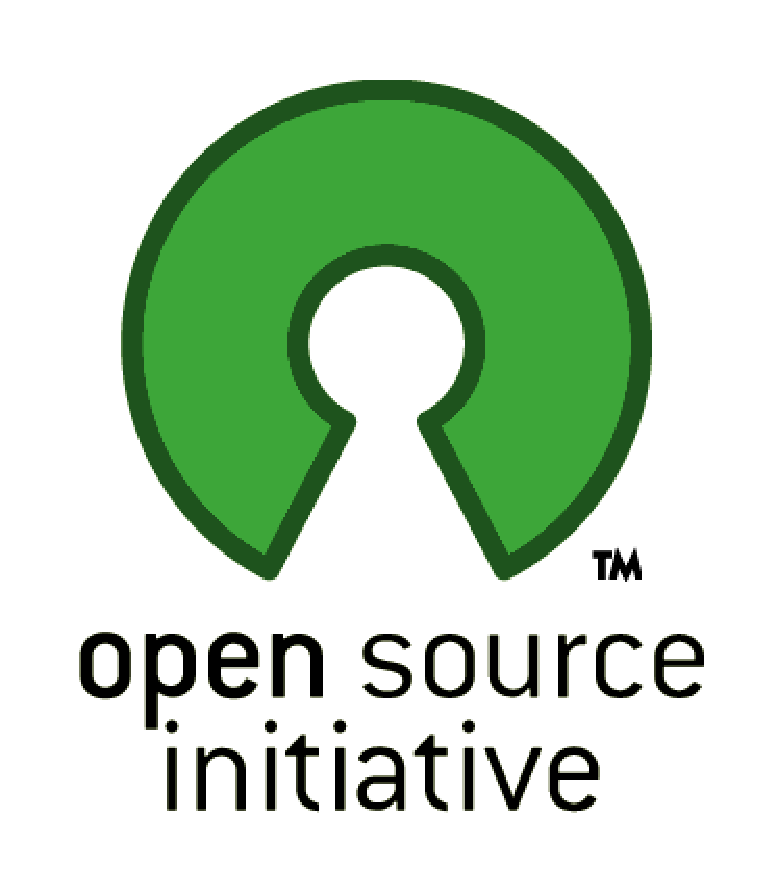
\includegraphics[scale=0.2]{img/intro/osi.eps}
	\caption[Open Source Initiative Logo]{Open Source Initiative Logo}
	\end{center}
\end{figure}


The idea of creating common software, of aiding other investigators to easily replicate the work already done and continue from that point instead of "reinventing the wheel" started in the past century. In 1998 the Open Source Initiative (OSI)\cite{osi} was formed, and its definition is recognized as the standard. According to them, "Open source does not just mean access to the source code. The distribution terms of open-source software must comply with the following criteria: Free Redistribution, Source Code, Derived Works, Integrity of The Author's Source Code, No Discrimination Against Persons or Groups, No Discrimination Against Fields of Endeavor, Distribution of License, License Must Not Be Specific to a Product, License Must Not Restrict Other Software,  License Must Be Technology-Neutral"\cite{osi_def}. 
\\

Open Source is crucial in the development of new knowledge and not only in the Software field, but in all the science and technical disciplines. 



